%*******************************************************************************
%****************************** Second Chapter *********************************
%*******************************************************************************

\chapter{A new Peierls model}
\label{chap:peierls_model}
\graphicspath{{peierls_model/Figs/}}


Though there are a number \cite{Nabarro1947,Huntington1955, puls1976, Vitek1992,  Bulatov1997, Lubarda2007, Clegg2006,Gouriet2015} of Peierls models in the literature published over the decades since \citet{Peierls1940} first presented his short solution few have been adaptable to situations beyond the initially envisaged problem which is typically narrowly defined. In this chapter such a model is presented that allows, with a minimum of effort, the consideration of energies defined by linear elasticity, empirical potentials, generalised stacking fault energies and could feasibly be extended to a full quantum mechanical treatment with density functional theory.

The python programming language was chosen for a number of reasons, firstly the python model is inherently modular, which provides a flexible structure, allowing parts of the model to be altered, extended or replaced quickly easily. Python is also widely used with a large body of documentation and a large support community. Finally python has a very large number of extending modules providing advanced capabilities, particularly projects like NumPy and SciPy. NumPy provides a powerful and efficient implementation of arrays providing a range of simple functions as well as more advanced linear algebra operations. SciPy is a project built on the basic data structure of the numpy array and provides advanced algorithms and convenience functions including differential equations, numerical solvers and optimisers, image processing and statistical functions.


To calculate the Peierls stress we must find the energy of dislocation configurations as the dislocation is displaced from one equilibrium position to the next. The variable $\alpha$ is used to denote the fractional displacement of the dislocation. Since boundary conditions are insufficient to define the atomic configuration, for each value of $\alpha$ the atomic configuration of the dislocation that minimises the energy must be found. Once a sufficient samples of $\alpha$ have been made the Peierls stress can be calculated by 

\begin{equation}
\tau_p = \frac{1}{lb^2}   \left. \frac{\partial U}{\partial \alpha} \right|_{max} .
\end{equation}

Where $l$ is the length of dislocation line for which the energy, $U$, is calculated for and $b$ is the Burgers vector.

So for a given value of alpha how can the ideal, that is lowest energy, configuration be found? This requires two steps, first the definition, creation and representation (as a data structure) of a configuration and second the evaluation of the energy thereof.
Taken together these can be thought of as a simple function that takes the value of $alpha$ along with some input parameters as arguments and returns the energy:

\begin{equation}
U = f(\alpha, p_1, p_2,...,p_n )
\label{eqn:energy_as_function}
\end{equation}

The input parameters, $p_i$, could be as general as the coordinates of every atom in the configuration or as specific as the single parameter defined by by Peierls in his original treatment, the width of the dislocation, the only difference is one of computational tractability. Algorithms exist for finding the minimum of functions of the form given in \autoref{eqn:energy_as_function} but they are much faster for functions with small numbers of parameters and some algorithms are not reliable for large numbers of parameters, hence decisions about how to define an atomic configuration will have consequences for the optimisation of that configuration.

Since a less general case can usually be taken to be a specific case of a more general one it seems sensible to use the most general representation of a dislocation and then apply constraints to it rather than find the model limited by an assumption of specificity later. Hence individual atoms are represented in space by coordinates as an array of the form:

$$ atoms = \begin{pmatrix}
x_1 & y_1 & z_1  \\
x_2 & y_2 & z_2  \\
.   &.    &.     \\
.   &.    &.     \\
x_n & y_n & z_n  \\
\end{pmatrix}
$$

Where $x$, $y$ and $z$ are coordinates in euclidean space in units of \r{A}ngstr\"{o}ms, i.e. \emph{not} relative to any crystallographic axes.

This representation can be extended, for example in the case of ionic solids the charge on each ion would be a necessary parameter for any energy calculation, this would be represented thus:
$$
atoms = \begin{pmatrix}
x_1 & y_1 & z_1 & q_1 \\
x_2 & y_2 & z_2 & q_2 \\
.   &.    &.    &.    \\
.   &.    &.    &.    \\
x_n & y_n & z_n & q_n \\
\end{pmatrix}
$$
This could be extended to an arbitrary number of parameters such as parameters for empirical potentials, labels for symmetrical distinct ions of the same species etc.





\section{Building a dislocation}
\FloatBarrier
\label{sec:build}




The model might be expected to start in the same way as Peierls; bringing together two half crystals as shown in \autoref{fig:semi_infinite_crystals} and simply allowing the structure to relax, leaving all the atomic positions as free variables. However there are two reasons to apply constraints to the atomic coordinates: firstly constraints reduce the number of parameters to search and secondly an unconstrained global optimisation might remove the dislocation entirely. This would create a perfect crystal, which would have a lower energy than a dislocated crystal. To achieve this a displacement field based on initial atomic coordinates is used to find a final atomic configuration.

For a given value of $\alpha$, there will be an initial configuration of atoms defined by two half crystals brought together at a slip plane with some relative displacement between them defined by $\alpha$ and the Burgers vector. The core of the dislocation is taken to be the line where $x,y = 0$. The position of the core with respect to the lattice of the half crystals is defined by $\alpha$, usually with $\alpha=0$ defining the configuration in which the extra half-plane of atoms aligns with the dislocation core, as shown in \autoref{fig:joined_half_crystals}. 

The final, in the sense of ready to be evaluated energetically rather than optimised, configuration is the combination of  the initial positions and an array of displacements defined by some displacement field, $\bm{\delta}(x_0, y_0, z_0)$, i.e.
\begin{equation}
\mathbf{r}_i = \mathbf{r}_i^0 + \bm{\delta}(\bm{r}_i^0)
\end{equation}
where $\mathbf{r}_i$ is the position vector defining the final position of the $i$th atom, $\mathbf{r}_i^0$ is the vector defining the initial position of the $i$th ion and $\bm{\delta}$ is a vector displacement field.


%%%%%%%%%%%%%%%%%%%%%%%%%%%%%%%%%%%%%%%%%%%%%%%%%%%%%%%%%%%%%%%%%%%%%%%%%%%5
%
%                      Initial half crystals
%
%%%%%%%%%%%%%%%%%%%%%%%%%%%%%%%%%%%%%%%%%%%%%%%%%%%%%%%%%%%%%%%%%%%%%%%%%%%%%%
\subsection{Defining the initial atomic positions}


Firstly we must define the initial positions of the atoms in the half crystals. In the Peierls model the material was assumed to be a simple orthorhombic lattice; i.e. a misaligned  bond across the slip plane has a minimum energy when the bond is normal to the slip plane. To consider the effects of the particular structure the atomic configuration must be generated from the lattice and motif of the perfect crystal.

To create a crystal conveniently oriented with respect to the Cartesian reference axes and the crystal slip system, unconventional unit cells were defined. Directions and planes defined relative to the unconventional or dislocation cell will be marked prime, e.g. $[1\,0\,0]'$. The Burgers vector $\mathbf{b}$ is taken to be the $[1\,0\,0]'$, the shortest slip plane normal that is a full lattice vector is taken to be $[0\,1\,0]'$ and the $[0\,0\,1]'$, parallel to the line vector, is the shortest lattice vector that is perpendicular to both the Burgers vector and the slip plane normal and its sign is such that the axes are right handed. Filling space by combining a motif and a lattice defined according to these axes is convenient because most of the mathematical results of dislocation theory, stress and strains fields etc., are defined taking $x$, $y$ and $z$ parallel to $[1\,0\,0]'$, $[0\,1\,0]'$, $[0\,0\,1]'$ respectively.

For example the \ce{NaCl} <1\,\={1}\,0>\{1\,1\,0\} slip system gives a new unit cell aligned with the slip system:

\begin{equation*}
\begin{aligned}[c]
{[1\,0\,0]}' &=\, ^{1}\!/_{2} [1\,1\,0]   \\
{[0\,1\,0]}' &=\, ^{1}\!/_{2} [1\,\overline{1}\,0]   \\
{[0\,0\,1]}' &=\, [0\,0\,1]   
\end{aligned}[c]
\qquad
\begin{aligned}[c]
&\parallel \mathbf{b} \\
&\parallel \mathbf{d} \\
&\parallel \mathbf{l}
\end{aligned}
\end{equation*}
where $\mathbf{l}$ is the line vector of the dislocation.


The atoms in this non-conventional unit cell are
$$
motif = \begin{pmatrix}
0 & 0 & 0 & +1 \\
^{1}\!/_{2} & ^{1}\!/_{2} & ^{1}\!/_{2} & +1 \\
0 & 0 & ^{1}\!/_{2} & -1 \\
^{1}\!/_{2} & ^{1}\!/_{2} & 0 & -1 \\
\end{pmatrix}
$$
where a $+1$ in the final column denotes the positive charge of a sodium ion and a $-1$ denotes the negative charge of a chloride ion.



\begin{figure}
\centering


    \begin{subfigure}{0.55\textwidth}
    \centering
    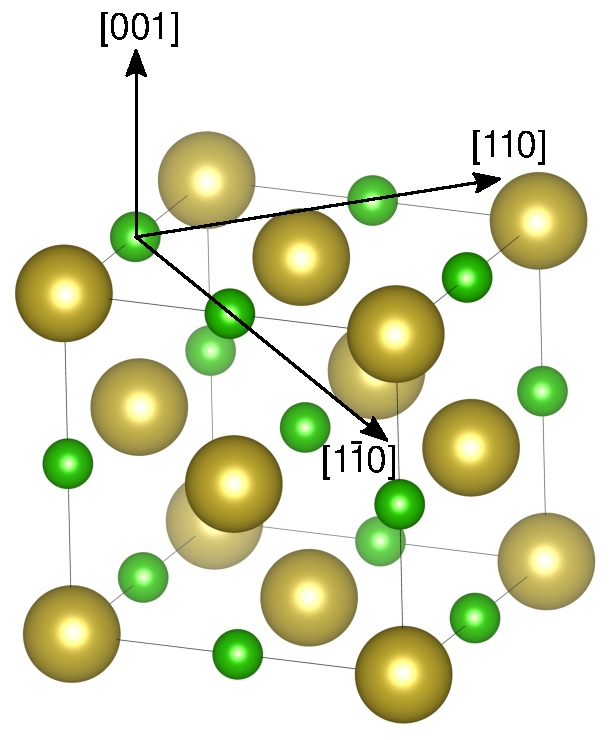
\includegraphics[width=\textwidth]{NaCl_conventional_unit_cell}
    \caption{The conventional unit cell of sodium chloride with the salient slip directions and plane normals highlighted. \label{fig:NaCl_conventional_cell_slip_system_marked}}
    \end{subfigure}

    \begin{subfigure}{0.4\textwidth}
    \centering
    \includegraphics[height=2.0in]{NaCl_110_110}
    \caption{The sodium chloride unit cell best aligned with the <1\,1\,0>\{1\,\={1}\,0\} slip system. \label{fig:NaCl_110_110_unit_cell}}
    \end{subfigure}
    ~
    \begin{subfigure}{0.4\textwidth}
    \centering
    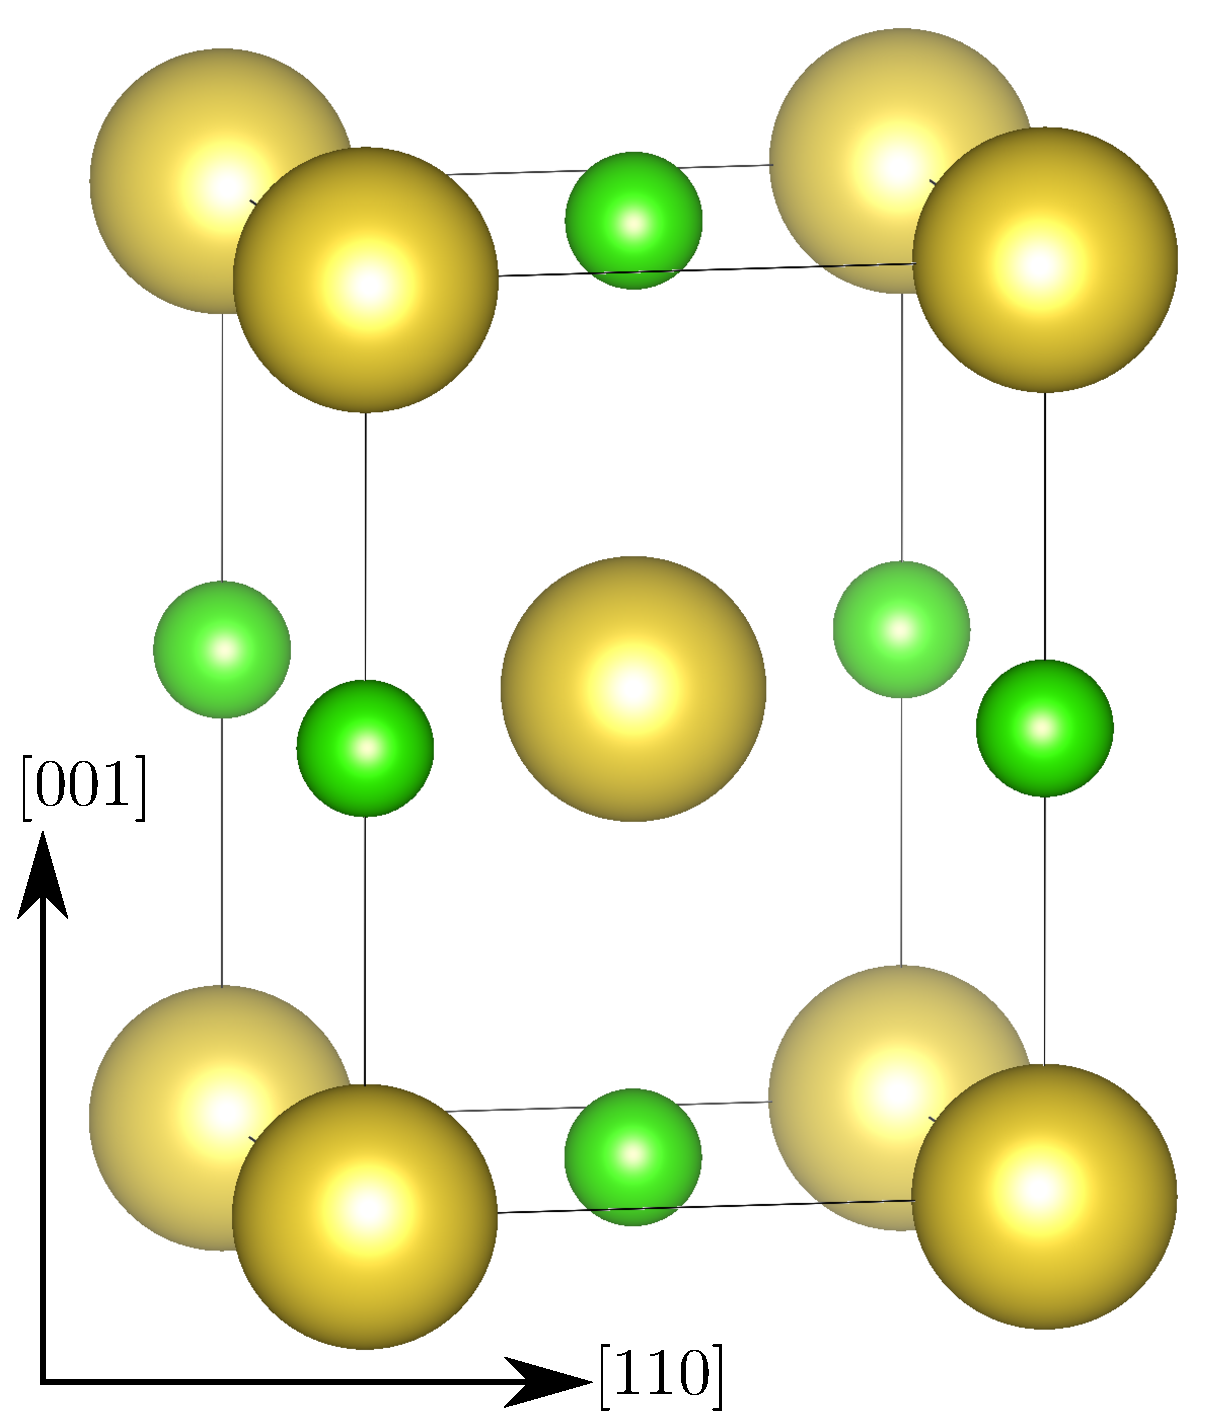
\includegraphics[height=2.5in]{NaCl_110_001}
    \caption{The sodium chloride unit cell best aligned with the <1\,1\,0>\{0\,0\,1\} slip system. \label{fig:NaCl_110_001_unit_cell}}
    \end{subfigure}

\caption[Unconventional unit cells of rock salt to build a dislocation.]{Possible unit cells for sodium chloride showing the conventional unit cell and two unconventional unit cells with the new crystallographic axes aligned to slip system, i.e. the Burgers vector and slip plane normal. Graphics prepared with VESTA \cite{Momma2011}.\label{fig:unconventional_NaCl_unit_cells}}
\end{figure}






Similarly the \ce{NaCl} <1\,\={1}\,0>\{0\,0\,1\} slip system is defined by the unit cell:
\begin{equation*}
\begin{aligned}[c]
 {[1\,0\,0]}' &=\, ^{1}\!/_{2} [1\,1\,0] \\
 {[0\,1\,0]}' &=\,  [0\,0\,1] \\
 {[0\,0\,1]}' &=\; ^{1}\!/_{2} [1\,\overline{1}\,0] \\
\end{aligned}
\qquad
\begin{aligned}[c]
&\parallel \mathbf{b} \\
&\parallel \mathbf{d} \\
&\parallel \mathbf{l}
\end{aligned}
\end{equation*}
and the atoms are
$$
motif = \begin{pmatrix}
0 & 0 & 0 & +1 \\
^{1}\!/_{2} & ^{1}\!/_{2} & ^{1}\!/_{2} & +1 \\
^{1}\!/_{2} & 0 & ^{1}\!/_{2} & -1 \\
0 & ^{1}\!/_{2} & 0 & -1
\end{pmatrix}
$$


These unit cells are shown in relation to the conventional cell in \autoref{fig:unconventional_NaCl_unit_cells}. With these unit cells we can convolve the motif with a lattice to generate an initially perfect crystal defined with respect to Cartesian axes aligned with the slip system. Two offsets are then applied; firstly the half crystal below the slip plane, which is defined by $y < 0$, will be offset in the positive $x$ direction by $b/2$ and then the entire crystal is offset to put the dislocation core in the desired location. The latter will require an offset along the slip direction, $[0\,0\,1]'$ of $\alpha b$ and an additional offset in the $[0\,1\,0]'$ direction. While the magnitude of this offset is not necessarily predictable, in the case of \ce{NaCl} the core must be at a height of $d/4$ in order to be halfway between the two (0\,2\,0) layers.

The initial positions of the atoms in the dislocated crystal are related to those of an initially perfect crystal by
\begin{equation}
\bm{r_i^0} = \bm{r_i^{\text{perfect}}} +\begin{cases}
[-\alpha{}b, h, 0] & \quad \text{if } y_i^{\text{perfect}} > 0\\
[b(1/2 - \alpha{}), h, 0] & \quad \text{if } y_i^{\text{perfect}} < 0\\
\end{cases} 
\end{equation}

The offset to the atomic coordinates in $-\alpha{}b$ such that as $\alpha$ increases the dislocation motion is in the positive $x$ direction.





\FloatBarrier












%%%%%%%%%%%%%%%%%%%%%%%%%%%%%%%%%%%%%%%%%%%%%%%%%%%%%%%%%%%%%%%%%%%%%%%%%%%%%%%%%%%

                          % Displacement fields

\subsection{Displacement fields}

A suitable displacement field is required. First we can take a Volterra dislocation, which in a continuous isotropic elastic medium has a displacement field \cite{Hirth1982Straight_dislocs}:
\begin{subequations}
\begin{align}
u &= \frac{b}{2\pi}\left[ \arctan\left(\frac{x}{y}\right) + \frac{xy}{2(1-\nu)(x^2 + y^2)} \right] \\[0.5ex]
v &= -\frac{b}{2\pi} \left[ \frac{1-2\nu}{4(1-\nu)} \ln(x^2 + y^2) + \frac{x^2 + y^2}{4(1-\nu)(x^2 + y^2)} \right]
\end{align}
\end{subequations}
where $u$ and $v$ are the components of the displacement field parallel to $x$ and $y$ respectively, $x$ is the initial position parallel to the Burgers vector, $y$ is the initial position parallel to the slip plane normal, $b$ is the magnitude of the Burgers vector and $\nu$ is the Poisson ratio of the material. The terms all converge to fixed values at large $x$ or $y$ except the logarithmic component of $v$. This represents the bending of a single crystal that arises from the introduction of an extra half plane \cite{Hirth1982Straight_dislocs}.

This formulation of the displacement field and subsequent solution for an isotropic elastic continuum is discontinuous, diverging at $r=0$, where $r=\sqrt[]{x^2+y^2}$. To remove the discontinuity \citet{Eshelby1949} proposed considering a single dislocation to be composed of a continuous distribution of dislocations with infinitesimal Burgers vectors, the integral of which yields the Burgers vector of the full dislocation. 

By considering the local strains (a normal strain parallel to the slip plane) due to this distribution, the stress on the slip plane can be found. By applying a force balance condition with the stress arising due to the misalignments, the displacements at the slip plane can be found, following the arguments laid out in \cite{Hirth_Lothe1982lattice_periodicity}. 

Let $\mathbf{b}'dx'$ be the Burgers vector of an infinitesimal dislocation lying between $x'$ and $x'+dx'$. The dislocation corresponds to a displacement of $-2(du/dx)dx'$. The total Burgers vector can be found by integration:
\begin{equation}
b = \int_{-\infty}^{\infty} b'(x') \dd x' = -2\int^{\infty}_{-\infty} \left( \! \frac{\dd u}{\dd x} \right)_{x=x'} \dd x' 
\end{equation}

The shear stress due to a Volterra dislocation  is \cite{hirth_lothe1982peierls_displacements}
\begin{equation}
\sigma^{\text{Volterra}}_{xy} = \frac{\mu b}{2\pi (1-\nu)} \frac{x(x^2 - y^2)}{(x^2+y^2)^2}
\end{equation}
where $x$ relates to the the core of the single dislocation, centred on the origin, with Burgers vector $b$.

The shear stress on the slip plane due to a single Volterra dislocation is found, by setting $y=0$ and substituting for $b$, to be
\begin{equation}
\sigma^{\text{Volterra}}_{xy}(x,0) = -\frac{\mu}{2\pi(1-\nu)} \int^{\infty}_{-\infty} \frac{b'}{x-x'} \!\dd x' =  \frac{\mu}{\pi(1-\nu)} \int^{\infty}_{-\infty} \frac{1}{x-x'} \left(\!\frac{\dd u}{\dd x}\right)_{x=x'} \!\dd x'
\label{eqn:elastic_stress_at_slip_plane}
\end{equation}
where $x-x'$ is the distance between some point $x$ and the infinitesimal dislocation at $x'$.

At the minimum energy position the net stress on the slip plane, i.e all $(x,0)$, vanishes, so there must be a balancing stress arising from the misalignment of the material across the slip plane. By analogy with \citet{Frenkel1926}:
\begin{equation}
\sigma_{xy}^{\text{misalignment}}(x,0) = C \sin \left( \frac{2\pi \phi}{b} \right)
\end{equation}
or in terms of the displacements either side of the slip plane:
\begin{equation}
\sigma_{xy}^{\text{misalignment}}(x,0) = -C \sin \left( \frac{4\pi u}{b} \right)
\end{equation}
If Hooke's law is satisfied at small strains we can write
\begin{equation}
\sigma_{xy}^{\text{misalignment}}(x,0) = 2 \mu \varepsilon_{xy} = \frac{\mu{}\phi}{d}
\label{eqn:misalign_stress_at_slip_plane}
\end{equation}
We can combine \autoref{eqn:elastic_stress_at_slip_plane} and \autoref{eqn:misalign_stress_at_slip_plane} to give an integral equation thus:
\begin{equation}
\int^{\infty}_{-\infty} \frac{1}{x-x'} \left(\!\frac{\dd u}{\dd x}\right)_{x=x'} \dd x' = \frac{b(1-\nu)}{2d} \sin\left(\frac{4\pi{}u}{b}\right)
\end{equation}
A solution is \cite{hirth_lothe1982peierls_displacements, Eshelby1949}
\begin{equation}
u(x) = -\frac{b}{2\pi} \arctan \left( \frac{x}{w} \right)
\label{eqn:one_dimensional_displacements}
\end{equation}
where $w$ is the half width of the dislocation and, for an isotropic elastic solid, has the value
\begin{equation}
w = \frac{d}{2(1-\nu)}.\label{eqn:half_width}
\end{equation}
\autoref{eqn:one_dimensional_displacements} satisfies the boundary condition that $u(\infty) = - u(-\infty) = -b/4$. $x=w$ gives $u(w)=1/2\, u(\infty)$, i.e. in the region $-w < x < w$ the disregistry across the slip plane is greater than half the maximum that occurs at $x=0$.

The two dimensional case gives a displacement field \cite{Eshelby1949,Leibfried1949,nabarro1987theory}:
\begin{subequations}\label{eqn:displacements}
\begin{align}
u(x,y) &= \frac{b}{2\pi} \left( \arctan \left[ \frac{y +  w\frac{|y|}{y}}{x} \right] - \frac{\pi}{2} \frac{|y|}{y} \frac{|x|}{x} \right) + c_1 \frac{xy}{x^{2} + (y + w\frac{|y|}{y} )^2} \\
v^y(x,y) &= c_2 \frac{y(y +  w \frac{|y|}{y})}{x^2 + (y +  w \frac{|y|}{y})^2} + c_3 \ln \left| \frac{x^2 + (y +  w \frac{|y|}{y})^2}{b^2} \right|
\end{align}
\label{eqn:displacement_field}
\end{subequations}
The final atomic configuration is then defined by 
\begin{equation}
\bm{r}_i = \bm{r}_i^0 + [u_i\,\bm{\mathrm{\hat{i}}},\; v_i\,\bm{\mathrm{\hat{j}}},\; 0\,\bm{\mathrm{\hat{k}}}]
\end{equation}

These terms can be interpreted physically: the arctan term is the same as in the original Peierls treatment, representing displacements along the slip plane that alter the local misalignment across the slip plane. The terms with the prefactors $c_1$ and $c_2$ represent shear strains: the $xy$ and $yx$ shears respectively. The logarithmic term, with the prefactor $c_3$, represents the bending of the entire crystal that must arise from the introduction of an extra half plane of atoms. This logarithmic term does not converge to a constant value at large $x$ or $y$, but this is consistent with this physical interpretation \cite{hirth_lothe1982peierls_displacements}.

Hence the parameters have physical interpretations: The width of the dislocation still defines the region with large disregistries, while $c_1$ and $c_2$ define the magnitude of displacements associated with shear strains around the dislocation core and $c_3$ defines the magnitude of the bending of a crystal that must arise from the introduction of an extra half plane of atoms.
To illustrate the displacements produced by these different terms some exaggerated (by a factor of ten from that predicted for an isotropic elastic medium) dislocation configurations are shown in \autoref{fig:parameters_of_the_disloc_configuration}.




\begin{figure}
\centering

    \begin{subfigure}{0.4\textwidth}
    \centering
    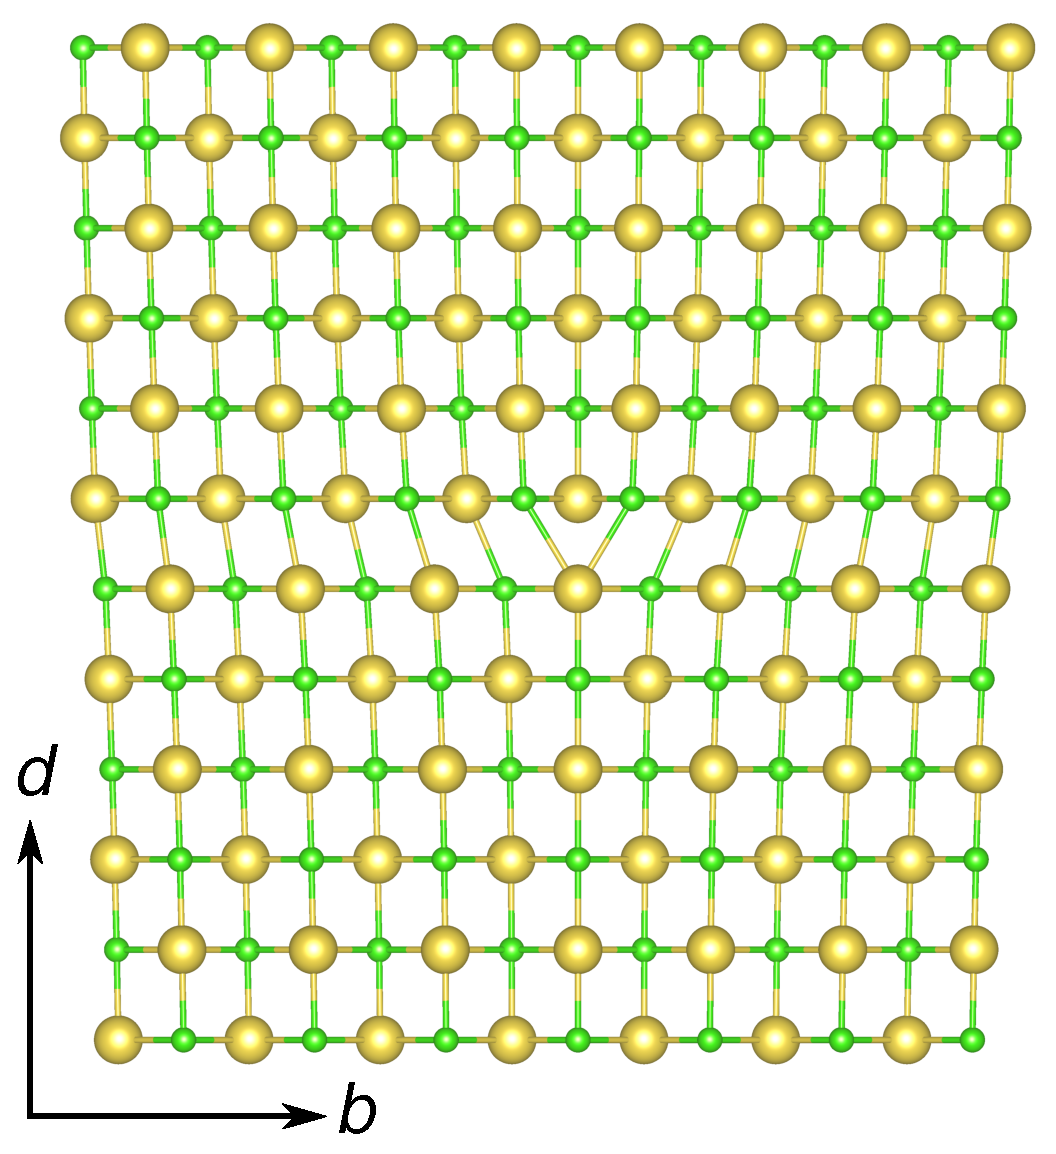
\includegraphics[width=0.6\textwidth]{wide_NaCl}
    \caption{A dislocation with a large width.}
    \end{subfigure}
    ~
    \begin{subfigure}{0.4\textwidth}
    \centering
    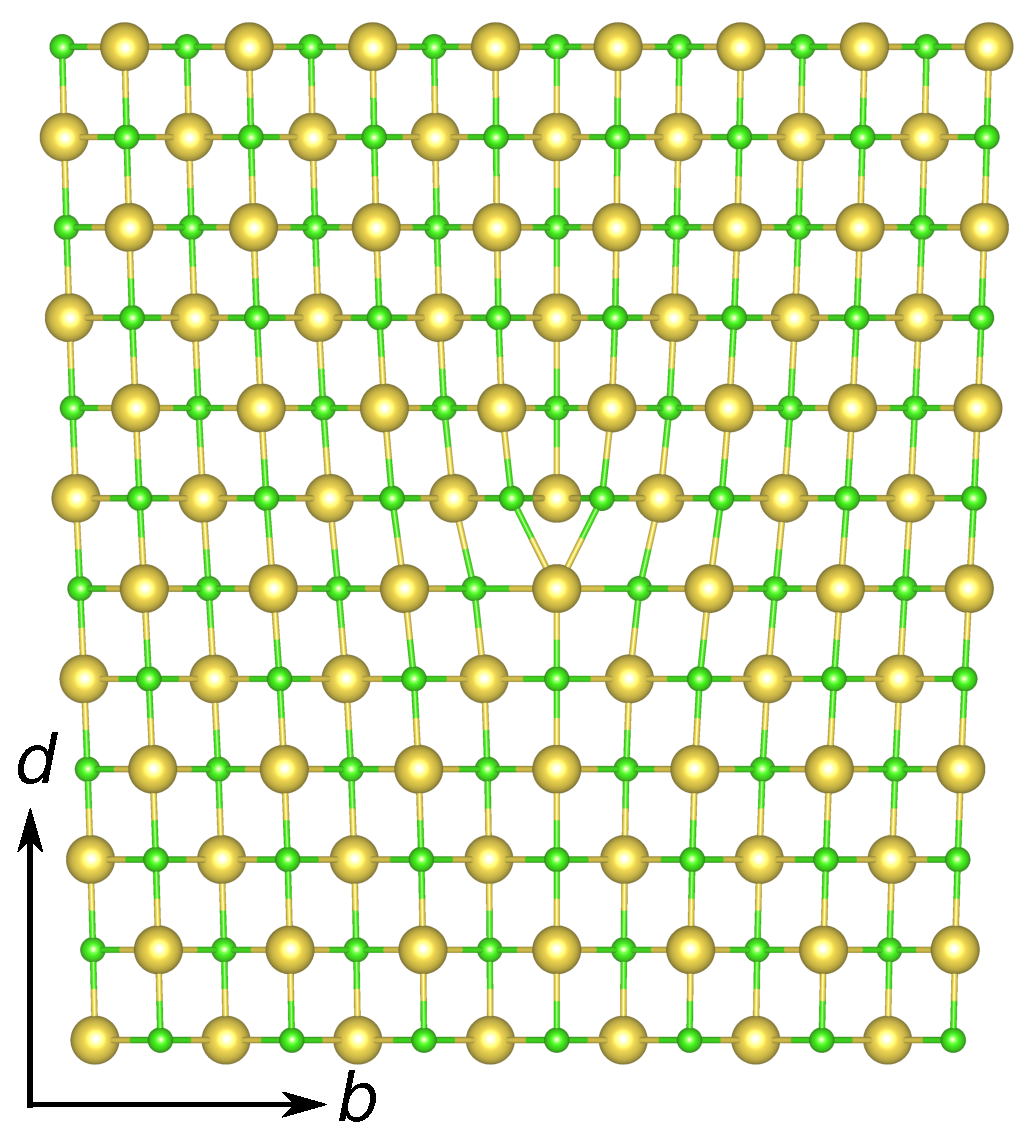
\includegraphics[width=0.6\textwidth]{narrow_NaCl}
    \caption{A dislocation with a small width.}
    \end{subfigure}

	\begin{subfigure}{0.4\textwidth}
	\centering
    \includegraphics[width=0.6\textwidth]{large_c1_NaCl}
    \caption{Large values of $c_1$ and $c_2$.}
	\end{subfigure}
    ~
	\begin{subfigure}{0.4\textwidth}
	\centering
    \includegraphics[width=0.6\textwidth]{large_c3_NaCl}
    \caption{A large value of $c_3$.}
	\end{subfigure}

    \begin{subfigure}{0.8\textwidth}
    \centering
    \includegraphics[width=0.5\textwidth]{typical_NaCl}
    \caption{A ``typical'' configuration.}
    \end{subfigure}

\captionsetup{width=0.8\textwidth}
\caption[The displacement field around an edge dislocation in rock salt.]{Various configurations of sodium chloride <1\,1\,0>\{0\,0\,1\} dislocations demonstrating the effects of the parameters of the displacement field defined in \autoref{eqn:displacements}, $w$, $c_1$, $c_2$ and $c_3$. Typical parameters are taken to be those predicted for an isotropic elastic material as given in  Equations~\ref{eqn:half_width} and \ref{eqn:disloc_params}, giving \SI{1.78}{\angstrom}, \SI{0.40}{\angstrom}, \SI{0.40}{\angstrom} and \SI{-0.12}{\angstrom} respectively for sodium chloride. Exaggerated values were ten times that. Calculated with $\nu =$~\num{0.207} and $a =$~\SI{5.644}{\angstrom} \cite{Theocaris1994,Rao1990}. Graphics prepared with VESTA \cite{Momma2011}.\label{fig:parameters_of_the_disloc_configuration}}
\end{figure}


The inclusion of $v(x,y)$ in the displacement field means that there will always be some finite displacement normal to the slip plane. This is expected and is be associated with phenomena such as pressure dependent yield stress \cite{frost1982pressure}. These displacements might also be responsible for the normal strains observed around line defects in layered crystals that have been ascribed to  a new class of defect called ripplocations \cite{Gruber2016}.




For an isotropic elastic medium the various parameters in \autoref{eqn:displacement_field} are found analytically  to have fixed values for the lowest energy dislocation. The half-width, $w$, takes the same value as in \autoref{eqn:half_width} and the three other parameters are defined by
\begin{subequations}\label{eqn:disloc_params}
\begin{align}
c_1 &= \frac{b}{4\pi{}(1-\nu)} \\
c_2 &= \frac{b}{4\pi{}(1-\nu)} \\
c_3 &= - \frac{b(1-2\nu)}{8\pi(1-\nu)}.
\end{align}
\label{eqn:expressions_for_the_ideal_disloca_parameters}
\end{subequations}
The terms of the form $|x|/x$ and $|y|/y$ are to give all the terms the right sense in the right regions of space, i.e. above and below the slip plane in $y$ and either side of the dislocation in $x$. This reduces to the simpler solution in \autoref{eqn:one_dimensional_displacements} if only the atoms adjacent to the slip plane are considered. This form is useful because it is continuous and finite for all values of $x$ and $y$. 


This gives a displacement field for a general material  which has four parameters: the width, $w$, and the scaling factors, $c_1$, $c_2$ and $c_3$. These parameters are varied to find the lowest energy dislocation. If the energy is calculated by an atomistic model, rather than by continuum elasticity, then there is no analytical solution for these parameters. Instead those values that minimise the energy are taken to be the correct solution.







A final note on the parametrisation of the dislocation structure is that the values $c_1$, $c_2$ and $c_3$ are not constrained. The purely isotropic case described above the parameters $c_1$, $c_2$ are positive and $c_3$ is negative, but there is no physical reason they cannot have a different sign. However a negative value of the width is not physically meaningful in this formulation. A negative width reintroduces the discontinuity at which displacements would diverge (in fact it would introduce two, one either side of the slip plane). Hence the constraint that $w>0$ is applied, but $c_1$, $c_2$ and $c_3$ are allowed to vary freely.





































\section{Evaluating the dislocation energy}
\label{sec:dislocation_energy}



Since there are insufficient boundary conditions to completely define a dislocation configuration with even four parameters the energy of the dislocation is the only way to identify a``correct'' or true configuration. Hence we must characterise the energy of arbitrary configurations. One obvious method to calculate the energy is to try and replicate the model based on elastic energy in the two half crystals and misalignment energy across the slip plane, there is the opportunity to calculate the full strain tensor and along with single crystal elastic constants the effects of elastic anisotropy can be taken into account. Another would be to use empirical potentials similar to those used in molecular dynamics; this would allow the exploration of dislocation properties in materials that are not well modelled by elasticity, ionic solids or compound semiconductors are examples of materials where elasticity is probably less appropriate. Both of these approaches are explored.

\subsection{Strain energy and misalignment energy}

This approach builds on the original approach of \citet{Peierls1940} and then \citet{Nabarro1947} and explains how the dislocation is stable due to a balancing of two forces, there is a force that attempts to spread the dislocation out into a planar defect, this arises due to the elastic stored energy in the bonds either side of the slip plane which would be zero in the case of a planar defect, which can be described by an infinitely wide dislocation. The other force tends to narrow the dislocation, this arises due to the misfit or misalignment across the slip plane. This would be a maximum for the planar defect where the entire slip plane is misaligned and would decrease monotonically as the width decreases.

Using this approach to the energy has a number of advantages. A two dimensional model is sufficient since for a long dislocation the condition of plane strain can be applied. If elastic theory can be applied at the scale of the unit cell then displacements need only be considered between unit cells rather than within them, which simplifies the model considerably.

\subsection{Strain energy}

Firstly the elastic energy can be easily calculated for a small volume if the strain and the elastic tensor is known. A good discussion of tensors and elasticity is given by \citet{kelly_knowles2012chapter5_tensors,kelly_knowles2012chapter6_stress_strain} and a discussion of elasticity in the context of dislocation theory is given by \citet{hirth_lothe1982elasticity}. The salient results are drawn together here.

Hookes law can be written as a tensor relationship using the einstein summation convention:
\begin{equation}
\sigma_{ij} = c_{ijkl} \epsilon_{kl}
\end{equation}
where $\sigma_{ij}$ is the stress tensor, $c_{ijkl}$ is the elastic tensor defining the properties of the material and $\epsilon_{kl}$ is the strain tensor. Strain is defined, for $i=j$, by
\begin{equation}
\epsilon_{ii} = \frac{\partial u_i}{\partial x_i}
\end{equation}
and for $i\neq j$ by
\begin{equation}
\epsilon_{ij} = \frac{1}{2} \left( \frac{\partial u_i}{\partial x_j} + \frac{\partial u_j}{\partial x_i} \right).
\end{equation}
%In Voigt notation the equation can be written
%\begin{equation}
%\sigma_i = c_{ij} \epsilon_{j}
%\end{equation}
%where 
%\begin{equation}
%\sigma_i = \begin{bmatrix}
%\sigma_{11} \\
%\sigma_{22} \\
%\sigma_{33} \\
%\sigma_{23} \\
%\sigma_{31} \\
%\sigma_{12} 
%\end{bmatrix}
%\qquad\qquad
%\epsilon_i = \begin{bmatrix}
%\epsilon_{11} \\
%\epsilon_{22} \\
%\epsilon_{33} \\
%\gamma_{23} \\
%\gamma_{31} \\
%\gamma_{12} 
%\end{bmatrix}
%\end{equation}
%This allows the reduction of the $3\times3\times3\times3$ tensor $c_{ijkl}$ to a $6\times6$ matrix $c_{ij}$. Note that to preserve the symmetry across the leading diagonal in $c_{ij}$ the strain components for $i\neq j$ are defined by $\gamma_{ij} = 2 \epsilon_{ij}$.
If Hooke's law holds then the stored elastic energy per unit volume is
\begin{equation}
u_{\text{elastic}} =\, ^{1}\!/_{2}\, \sigma_{ij} \epsilon_{ij} =\, ^{1}\!/_{2}\, c_{ijkl} \epsilon_{ij} \epsilon_{kl}.
\end{equation}
Hence to find the elastic energy we must evaluate \({\partial u_i}/{\partial x_j}\) for $i, j = 1, 2, 3$.
Assuming that we consider displacements between unit cells, and not within them, and assuming an orthogonal lattice estimating the components of strain is not difficult. The  condition of plane strain constrains $\epsilon_{ij} = 0$ for $i\, \text{or}\, j=3$. In the $1$--$2$ (or $x$--$y$) plane the strains can be identified from the vectors between neighbouring unit cells. For simplicity a primitive lattice is assumed and these vectors can be conceived of as bonds.

For this simple case for each atom two bonds are identified, one to the nearest neighbour in the $x$~direction and one to the nearest neighbour in the $y$~direction as shown in \autoref{fig:bonds}. The simplest estimate of the stress components is
\begin{alignat}{2}\label{eqn:estimate_strains}
\left. \frac{\partial u_x}{\partial x}\right|_i &= \frac{\mathbf{p}_i \cdot \mathbf{\hat{i}}}{b} &\qquad\qquad
\left. \frac{\partial u_x}{\partial y}\right|_i &= \frac{\mathbf{q}_i \cdot \mathbf{\hat{i}}}{d} \nonumber\\
\left. \frac{\partial u_y}{\partial y}\right|_i &= \frac{\mathbf{q}_i \cdot \mathbf{\hat{j}}}{d} &
\left. \frac{\partial u_y}{\partial x}\right|_i &= \frac{\mathbf{p}_i \cdot \mathbf{\hat{j}}}{b}
\end{alignat}


\begin{figure}
\centering
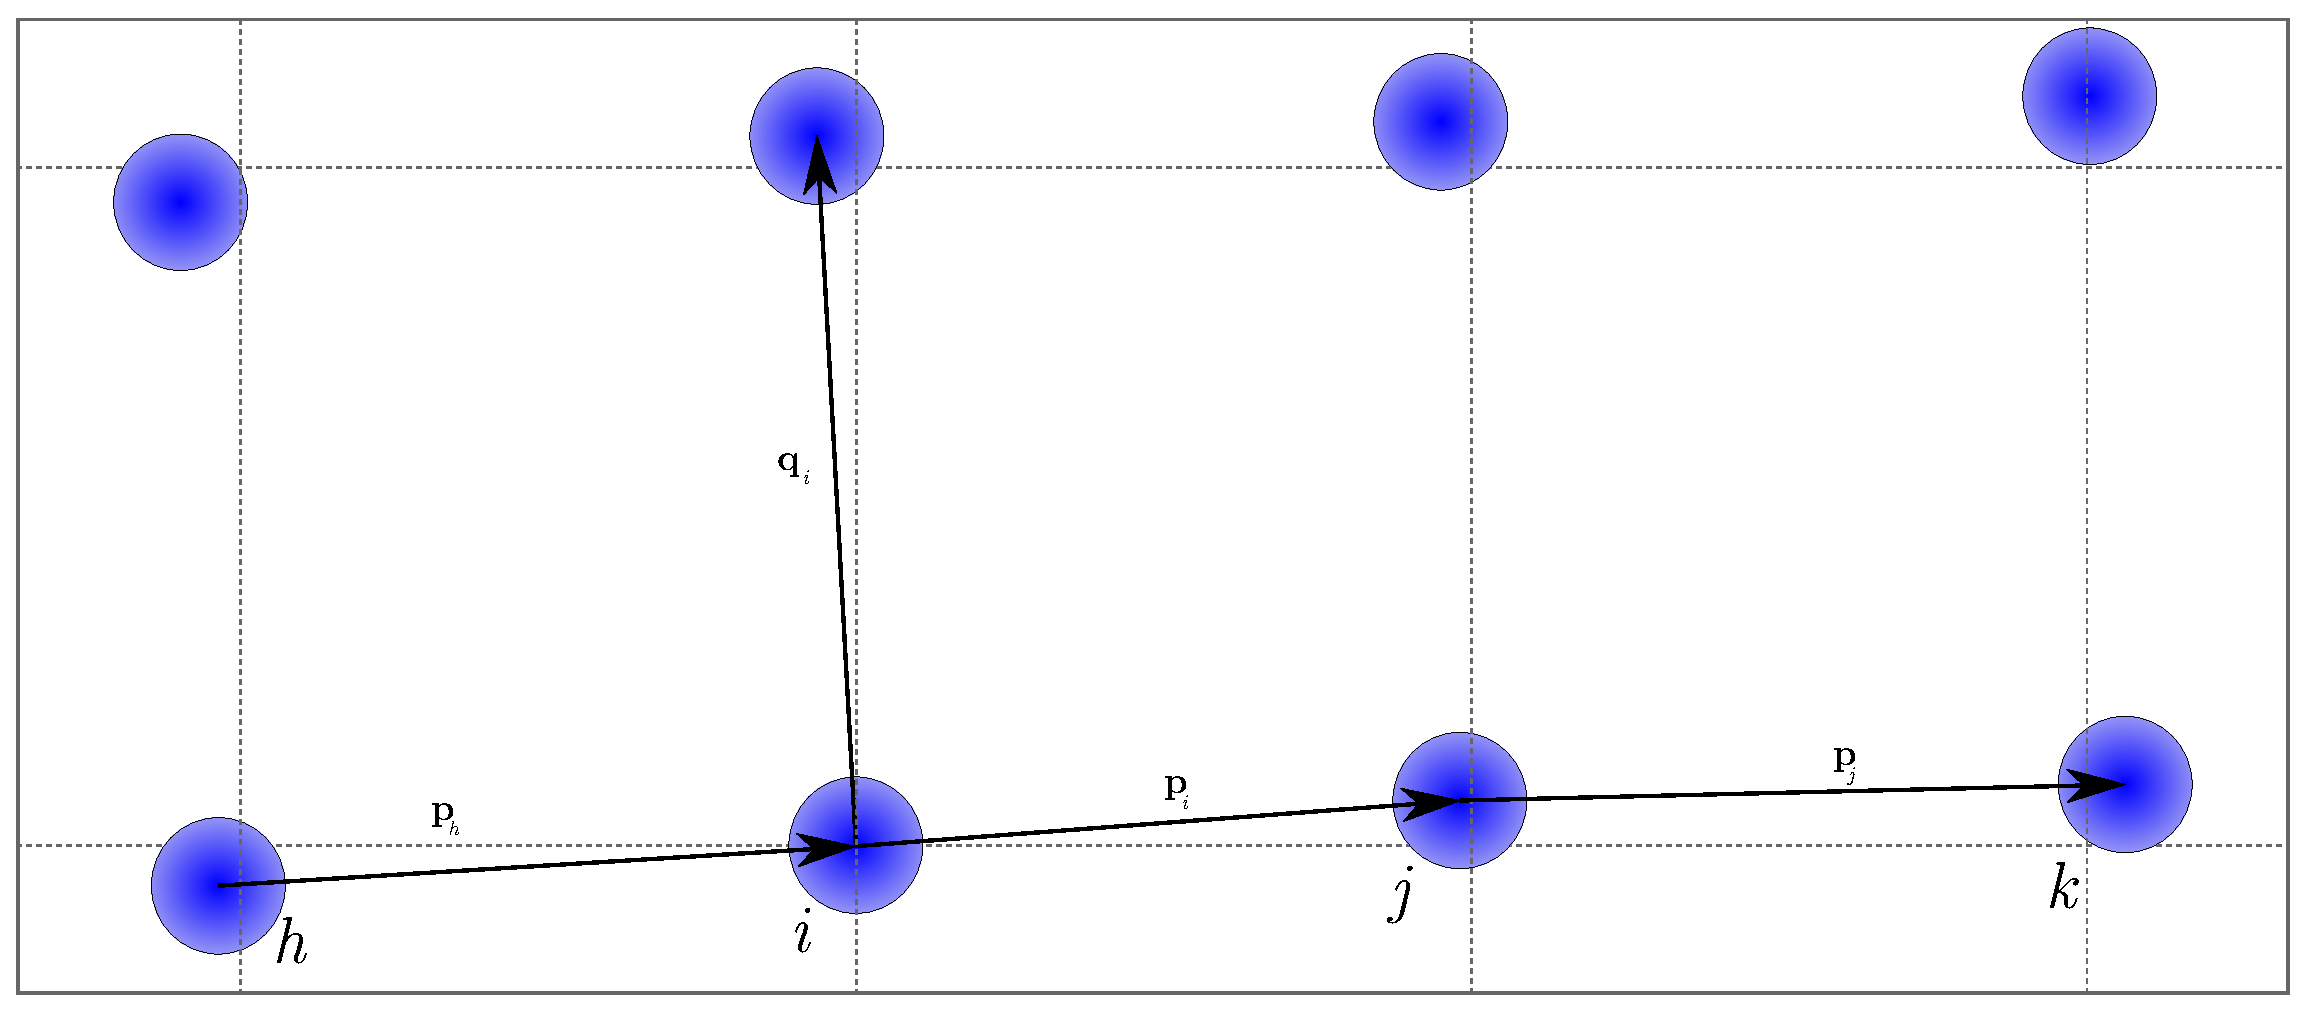
\includegraphics[width=\textwidth]{bonds}
\caption[Strained bonds in a dislocated crystal.]{The bonds that are considered for the $i$th atom in a region of crystal away from the slip plane; there is one bond to the nearest neighbour in the positive $x$~direction, $\mathbf{p}_i$, and one to the nearest neighbour in the positive $y$~direction, $\mathbf{q}_i$, to avoid double counting.\label{fig:bonds} }
\end{figure}





However there is a problem with this formulation. This assumes that every bond would, in equilibrium, be parallel to either the $x$ or the $y$ axis. This assumption is valid for the original Peierls model in which only displacements parallel to the $x$ direction were considered but the logarithmic term here represents a change in lattice orientation with position. A more nuanced approach requires some estimate of the local lattice orientation, if this is not done then the logarithmic term in \autoref{eqn:displacements} will mean that the strain in each bond will diverge, increasing with increasing distance from the dislocation core, whereas in reality the strains must be largest at the core.

There are clearly many possible ways of estimating the local lattice resistance, one possible method is to take the ideal orientation of the bond parallel to the slip plane for a particular bond to be paralell to the bonds on either side, i.e. as shown in \autoref{fig:bonds} the ideal orientation of $\mathbf{p}_i$ would be  parallel to $(\mathbf{p}_h + \mathbf{p}_j)$. The ideal orientation for $\mathbf{q}_i$ can be taken to be at \SI{90}{\degree} to this. So $\mathbf{\hat{i}}$ and $\mathbf{\hat{j}}$ in \autoref{eqn:estimate_strains} can be replaced with 
\begin{align}
\mathbf{\hat{i}}' &= \frac{(\mathbf{p}_h + \mathbf{p}_j)}{|\mathbf{p}_h + \mathbf{p}_j|} \nonumber \\
\mathbf{\hat{j}}' &= {\mathbf{\hat{i}}' \times \mathbf{\hat{k}}}
\end{align}
and the strain tensor can be calculated for each atom/unit cell, and hence the strain energy for each unit cell.



\FloatBarrier
\subsection{Misalignment energy}
\FloatBarrier

At the slip plane there is clearly going to be a break down of method highlighted above. For an atom immediately below the slip plane the identification of the nearest neighbour above the slip plane is perhaps not obvious. If the bond is taken to be simply  to the nearest atom above the slip plane ambiguities can arise 
It is possible that there will be two atoms equally close above the slip plane and such a simple criterion can lead to some atoms being bonded more than once and some atoms not being bonded. 

Instead a less arbitrary and more predictable method is to use the initial positions and assume that the $i$th atom can be bonded to two atoms in the layer above the slip plane. Since initially the horizontal spacing between atoms is $b$ for all atoms the two atoms must be within an interval $x_i^0 - b < x \leq x_i^0 + b$, as shown in \autoref{fig:slip_plane}. The energy for atom $i$ can be estimated from the average of the two bonds $\mathbf{q}_{i,\text{b}}$ and $\mathbf{q}_{i,\text{f}}$

\begin{figure}
\centering
\begin{subfigure}{\textwidth}
\centering
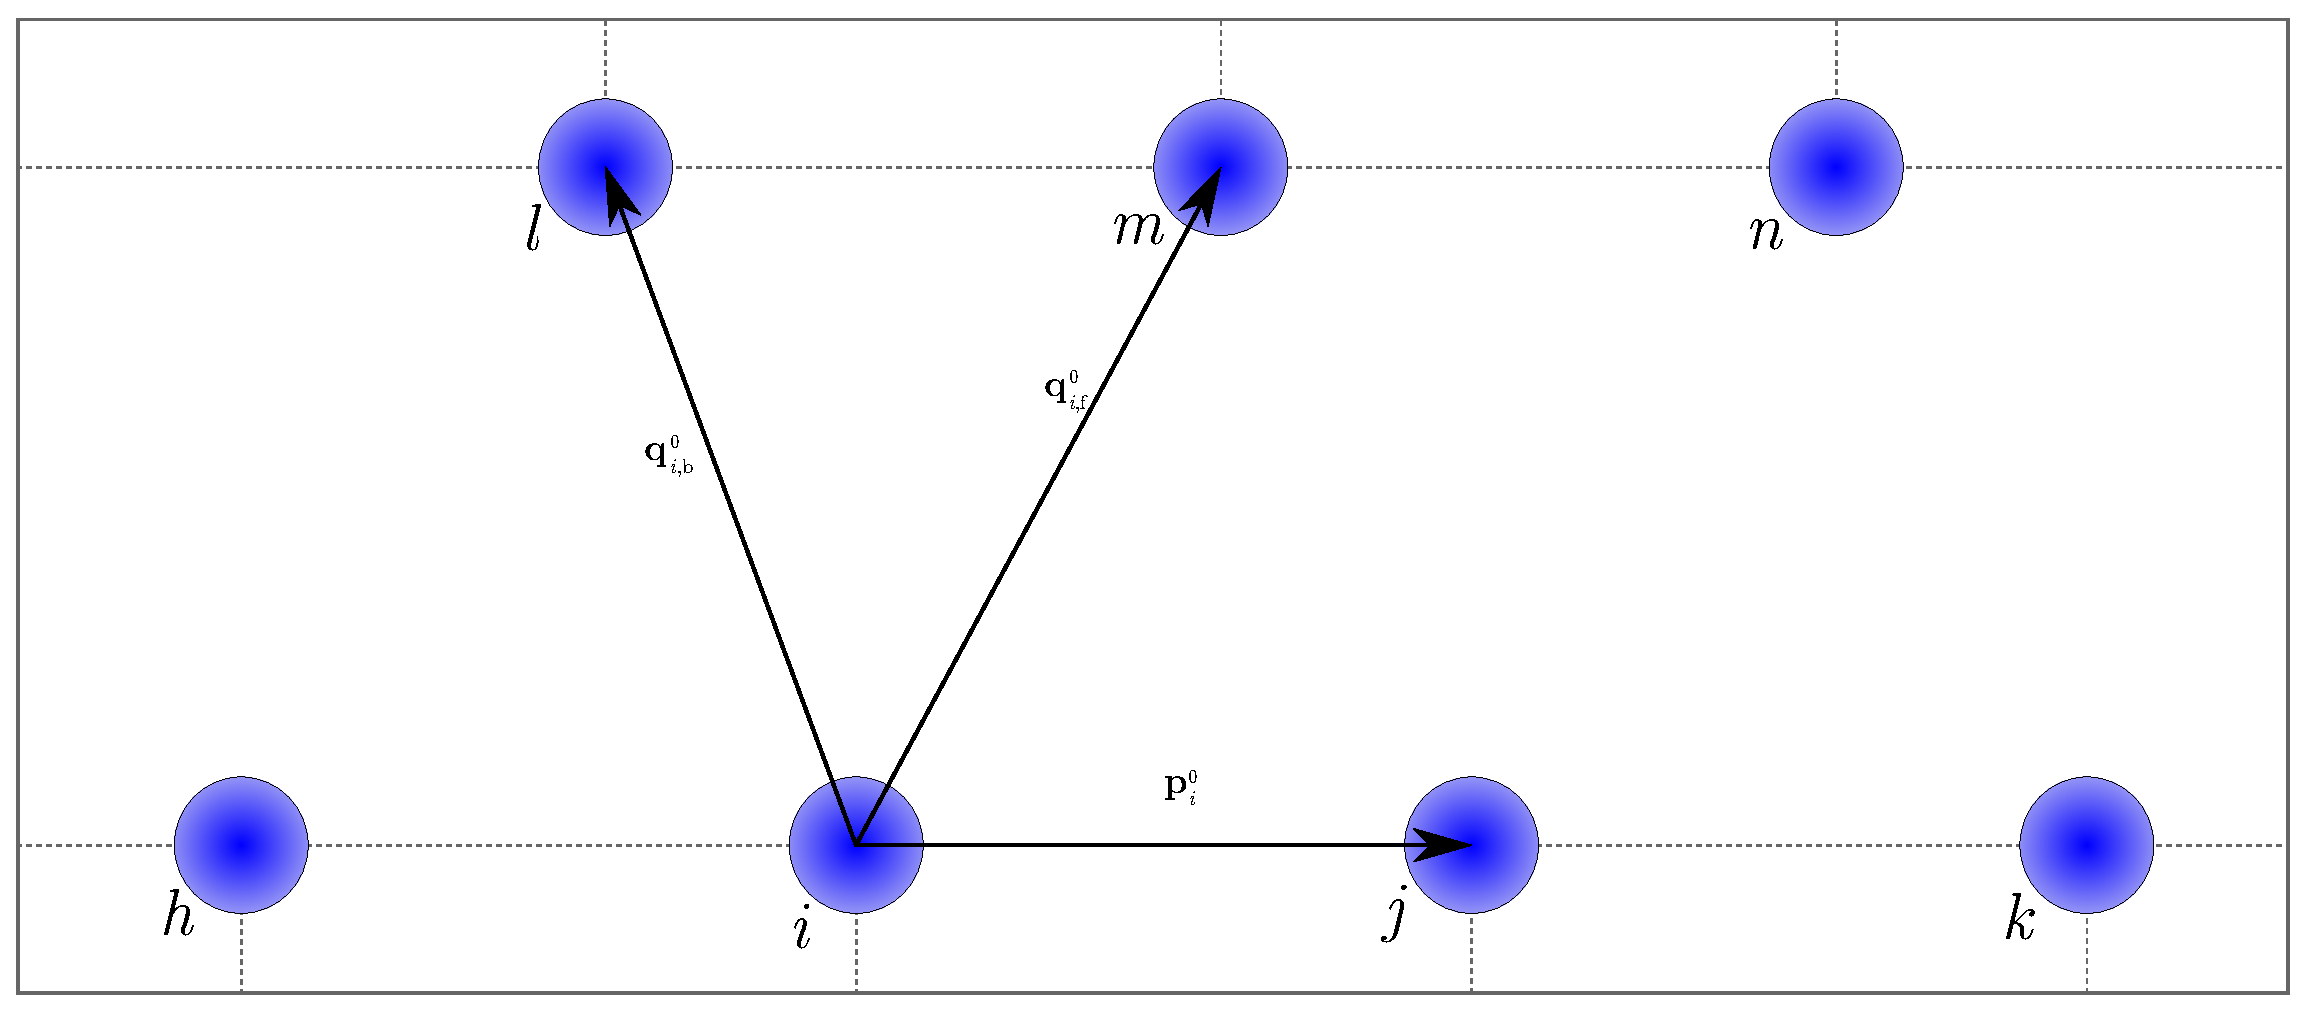
\includegraphics[width=\textwidth]{initial_slip_plane_bonds}
\caption{The initial positions of atoms either side of the slip plane.\label{fig:slip_plane_initial_positions}.}
\end{subfigure}
\par\medskip
\begin{subfigure}{\textwidth}
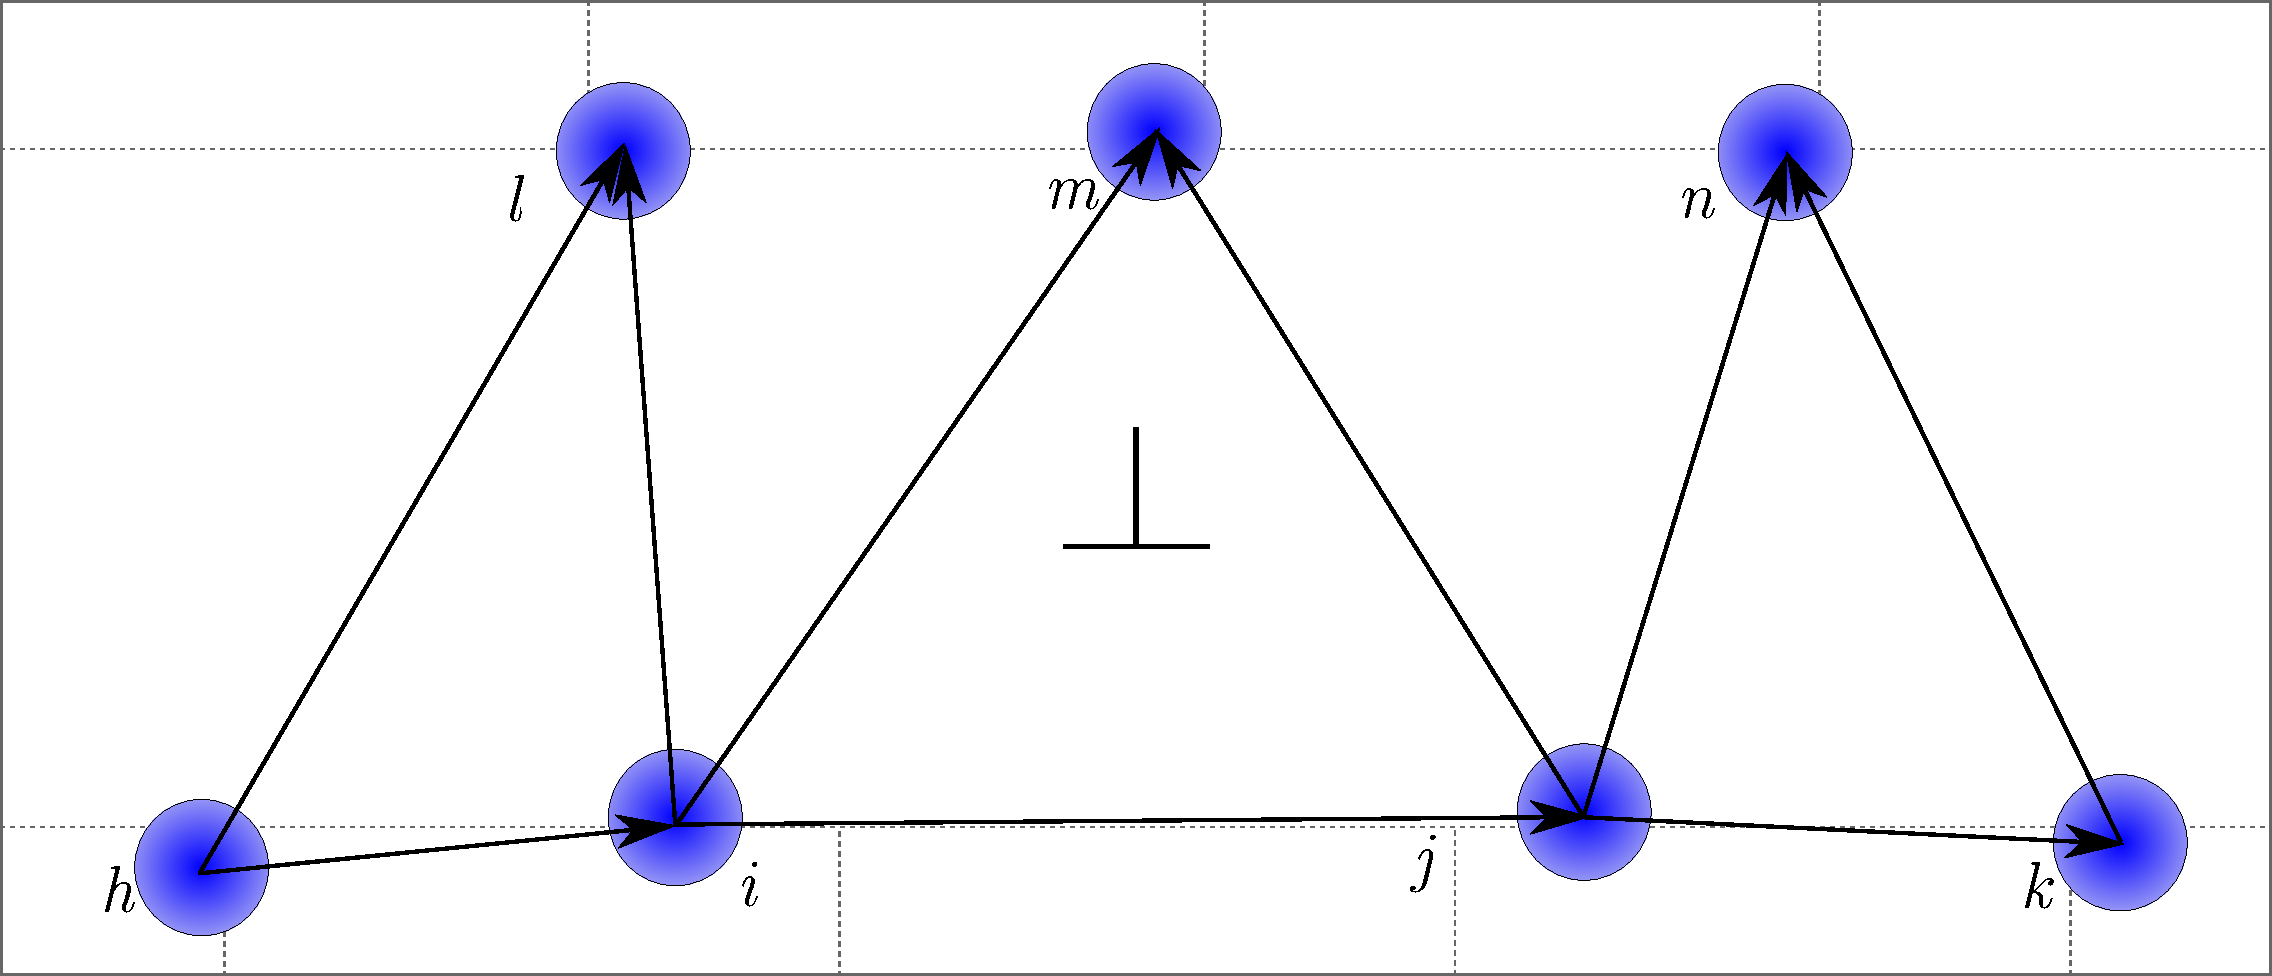
\includegraphics[width=\textwidth]{slip_plane_bonds}
\caption{The final positions of the atoms either side of the slip plane.\label{fig:slip_plane_final_positions}}
\end{subfigure}
\caption[Misaligned bonds cross the slip plane in a dislocated crystal.]{The slip plane before and after the application of the displacement field. The two atoms, $l$ and $m$, that can be considered bonded to the atom $i$ are shown along with the initial and final bonds, $\mathbf{q}_{i,\text{b}}$ and $\mathbf{q}_{i,\text{f}}$ which are backwards and forwards in the $x$ direction respectively. Also shown are the bonds $\mathbf{p}_h$ and $\mathbf{p}_j$ which are required to estimate the local orientation of the slip plane. \label{fig:slip_plane}}
\end{figure}


There are several methods to calculate the misaligned bonds. The simplest is to use the Frenkel approximation which, for an isotropic elastic material is 
\begin{equation}
U_i^\text{mis} = \frac{Gb^2}{4\pi^2} \left[\frac{d}{b}\right] \left[ 1 - \cos \left( \frac{2 \pi \phi}{d} \right) \right]
\end{equation}

which in terms of single crystal elastic constants takes $G=C_{66}$ (in Voigt notation see \cite{kelly_knowles2012chapter6_stress_strain}).

A more complete method for the calculation of the energy is to use the generalised stacking fault energy. Density functional theory can be used to calculate the energy of a stacking fault at an arbitrary misalignment. This is calculated by applying a displacement to two half crystals in a DFT simulation with periodic boundary conditions which introduces two opposing planar faults. The displacement is applied along the Burgers vector and the atoms are allowed to relax perpendicular to that displacement. Although the displacement field does not include any lateral (i.e. parallel to the lone vector) motion, allowing the DFT simulation of the stacking faults to relax laterally means that the energetic implications of lateral motion are included in the misalignment potential, although with an implicit assumption that the strains along the line vector do not extend beyond the slip plane. 

The energy changes with respect to a perfect crystal were considered and fitted with a simple empirical function:
\begin{equation}
\gamma(\phi) = \sum^{M}_{m=1} C_m \left[ 1 - \cos \left( \frac{2m\pi \phi}{b} \right) \right]
\end{equation}
where $\phi$ is the misalignment in the same units as the Burgers vector $b$, $m$ is an integer from \num{1} to $M$ and $C_m$ are coefficients fitted by a least-squares method to the energies calculated by DFT for different values of $\phi$. This is in units of \si{\joule\per\square\meter}, so a factor of $b$ must be applied to convert to a line energy in \si{\joule\per\meter}.


%%%%%%%%%%%%%%%%%%%%%%%%%%%%%%%%%%%%%%%%%%%%%%%%%%%%%%%%%%%%%%%5555%%%%%%%%%%%%%%%%%%%%%%%%%%%%%%%%%%%%%%%%%






%%%%%%%%%%%%%%%%%%%%%%%%%%%%%%%%%%%%%%%%%%%%%%%%%%%%%%%%%%%%%%%%%%%%%%%%%%%%%%%%%%%%%%%%%%%%%%%%%%%




\subsection{Empirical potentials}

Some materials can be described in a more physically insightful way than linear elasticity; as described in \autoref{sec:empirical_potentials}, empirical potentials have been developed for the field of molecular dynamics to be computationally convenient while at the same time approximating reality to a sufficient degree to gain insight into a system \cite{martinez2013}. One way to incorporate such potentials into the Peierls model described here is to write a simple python implementation of the potentials using the SciPy and NumPy packages and associated tools \cite{Numpy2011,Ipython2007,Millman2007,SciPy2001}; another way is to use the Atomic Simulation Environment \cite{ASE2017} or the python interface to the LAMMPS software package \cite{Plimpton1995,LAMMPS_web}.



To demonstrate the principle of using more physically informed potentials and hopefully capture more details of the energy changes as dislocations move the ionic solids were investigated using the Lennard-Jones potential:
\begin{equation}
\phi_{ij}(r_{ij}) = 4\epsilon_{ij} \left[ \left( \frac{\sigma_{ij}}{r_{ij}}\right)^{12}-     \left( \frac{\sigma_{ij}}{r_{ij}}\right)^6   \right]
\end{equation}
where $\epsilon_{ij}$ is the depth of the energy well and $\sigma_{ij}$ is the radius at which the energy is equal to zero or in the A--B form:
\begin{equation}
\phi_{ij}(r_{ij}) = \frac{A_{ij}}{r_{ij}^{12}} - \frac{B_{ij}}{r_{ij}^{6}}
\end{equation}
where $A_{ij} = 4\epsilon_{ij}\sigma_{ij}^{12}$ and $B_{ij} = 4 \epsilon_{ij} \sigma_{ij}^{6}$. The energy for any two atoms is then 
\begin{equation}
U_{ij}(r_{ij}) = \frac{1}{4\pi\epsilon_0} \frac{q_i q_j}{r_{ij}} + \frac{A_{ij}}{r_{ij}^{12}} - \frac{B_{ij}}{r_{ij}^{6}}
\end{equation}
where $\epsilon_0$ is the permittivity of free space.

The Lennard-Jones has been chosen as a simple example to demonstrate the application of empirical potentials for which fitted parameters are readily available \cite{Mao2014} and applicable to a class of materials for which the dislocation properties are not well explained by linear elasticity, the alkali halides.



\begin{table}
\centering
  \begin{tabular}{| m{3cm} | d{4} | d{-1} |}
  \hline
   Ion \rule{0pt}{3ex} & \multicolumn{1}{c|}{$\sigma_i$/\si{\angstrom}} & \multicolumn{1}{c|}{$\epsilon_i$/\si{\joule\per\mole}  }\\ \hline
   \ce{Li+} \rule{2ex}{0pt} & 1.715 & 241.25 \\
   \ce{Na+} & 2.497 & 327.44 \\
   \ce{K+} & 3.184 & 494.97 \\
   \ce{Rb+} & 3.302 & 1006.25 \\
   \ce{Cs+} & 3.440 & 2097.44 \\
   \ce{F-} & 3.954 & 27.05 \\
   \ce{Cl-} & 4.612 & 104.68 \\
   \ce{Br-} & 4.812 & 150.46  \\
   \ce{I-} & 5.197  & 176.56 \\
  \hline
  \end{tabular}
\caption[Lennard-Jones parameters.]{\rule[3ex]{0pt}{0pt} Parameters used for Lennard-Jones calculations from \cite{Mao2014}.\label{tab:LJ_params}}
\end{table}


The parameters used for the Lennard-Jones potential are shown in \autoref{tab:LJ_params}. They are calculated for each ion individually, to best reproduce lattice properties, and must be combined according to Lorentx-Berthelot rules:
\begin{align}
\epsilon_{ij} &= \sqrt[]{\epsilon_i \epsilon_j} \nonumber\\
\sigma_{ij} &= \frac{\sigma_i + \sigma_j}{2}
\end{align}

A na\"{\i}ve brute force implementation is given in Section~\ref{sec:ionic_energy_code} and an example input file is given for LAMMPS in Section~\ref{sec:lammps_input}. The LAMMPS pair style used was ``\texttt{lj/long/coul/long}'', the parameters for which are given in the example input file and is described in the LAMMPS documentation in \cite{LAMMPS_web}.

\subsection{Optimisation of the dislocation structure}
\label{sec:optimisers}
Given one of the above cases, or a similar one, that provides energy as a function of a small number of parameters, an optimisation routine is required. The original version of this Peierls model included a simple binary search algorithm to find the width of the dislocation. However for a multi-parameter space this is not appropriate.

Fortunately the open source project SciPy has a number of optimisers built in. The one chosen was the quasi-Newton method of Broyden, Fletcher, Goldfarb, and Shanno \citep{SciPy2001,nocedal2006}, or BFGS. This method uses the first derivative, methods such as this are known as hill-climbing optimisers, seeking a stationary point.

While the derivative of the energy with respect to the parameters is not simple to find, the atomic positions are defined as smooth functions of the input parameters and the energy is (at least likely to be) a smooth function of the atomic positions. Hence the overall behaviour of the energy as a function of the input parameters should be well suited to a gradient based method. The SciPy implementation of the BFGS algorithm includes the ability to approximate the first derivative numerically.

If it is found that the energy function is not well behaved SciPy also includes the Nelder-Mead simplex algorithm that does not make use of gradient information. This method calculates the objective function, here the energy, at $n+1$ points in parameter space where $n$ is the number of parameters. This defines a ``simplex'', i.e. a triangle in two dimensions, a tetrahedron in three and so on. A search direction is defined along the vector joining the worst of these $n+1$ points and the centroid of the rest, and a small number of point along this line are trialled. The worst point of the initial simplex is then replaced and the process repeated \citep{Nelder1965,Gao2012}.





































































